\chapter{Overview of Dark Matter research}
\label{chap:introDM}
For the past few decades, dark matter (DM) has been a concept of overwhelming interesting  given its ability to explain different aspects of cosmology in a single, nearly self-sufficient theory. %Dark matter could provide a single almost self sufficient theory to explain several observations in cosmology scale. 
Dark matter could be a crucial part of the history of revolution of the universe, which describes how our universe started from the initial mass density fluctuation, and evolved to its current status with the clusters, galaxies, super clusters, and other structures in various cosmological scales. %, the predicted abundance of Hydrogen, Helium and other light elements from nucleosynthesis.
It explains the amplitude of the temperature anisotropy spectrum in the cosmic microwave background (CMB), especially  the relative ratios of the amplitudes of the peaks on this spectrum.  It also explains several observations in the formation of the different scale structures in the universe. Dark matter also could explain the observations on the galactic scale, including the discrepancy in mass between luminescence (baryonic) mass and the weak lensing mass, as well as the weak lensing of CMB, the galactic rotation curves. Several other observations including the abnormally at \SI{3.5}{\keV} spectrum may also relate to the existence of dark matter. %Also recent research claim the observation of cooling of the $21 cm$ line is one of the evidence dark matter.

Based on these observations, researchers have proposed different theories for the form of dark matter. Non-relativistic (heavy mass) particle form dark matter (cold dark matter, CDM) has the advantage in its derived nature abundance via freeze-out theory at the early stages of the universe, and also that its low mobility allows for accumulating in cluster formation. However, relativistic particle dark matter is still being discussed, for its advantage in explaining the for explaining the formation of large-scale structures like big super clusters and voids at the scale of \SI{50}{\mega\parsec} in the space. In another formation theory of dark matter, for example, massive astrophysical compact halo objects (MACHOs), including black holes or neutron stars as well as brown dwarfs and unassociated planets, may also explain the discrepancy of the mass quantity in the galaxy halo.    

However, it might be dangerous to assume the same physics between the early days of the universe and now. Moreover, even though dark matter is a satisfyingly parsimonious explanation for several phenomena, it cannot be excluded that several other different explanations could exist for these problems. 

In this chapter, I will review the existing evidence for dark matter. I will also discuss about the candidates for the form of dark matter particles/objects. I will not attempt to cover the full history of both the observations and the detailed mathematical calculations in this thesis. The discussion here follows the more detailed treatment in Ref.~\cite{Bertone2005,Roos2010,Dodelson2003}. 

\section{Cosmological evidence for dark matter}
 \subsection{Evolution of the universe, density perturbation}
 According to some of the compelling theories and evidence of the  universe's evolution, the universe is currently expanding at an accelerating rate. We are on the stage of the acceleration of this expansion of the universe. The rate of the expansion of the universe is guided by the density of the universe in the curvature of space time. This leads to the famous Friedmann equations: 
\begin{align}
\label{freidmann}
\frac{\dot{a}^2+k}{a^2} &= \frac{8 \pi G \rho+ \Lambda}{3} \\
\frac{\ddot{a}}{a} &= -\frac{4 \pi G} {3}(\rho+3 p) + \frac{\Lambda}{3}
\end{align}  

Here, $a$ is the scale factor that describes the coherent distance of the universe. Conventionally, $a$ is taken to be $1$ at the present time.

$G$ is the Newton's gravitational constant(normal value is \SI{6.674e-11}{\cm\cubed\per\kg\per\second\squared}). Ref.~\cite{NIST}

$\Lambda$ is cosmological constant.

$k$ is the spatial curvature. If $k$ is positive, the shape of the universe is hyperspherical. If $k$ is negative, the shape of the universe is hyperbolic. And if $k$ is zero, then the universe is flat.
$\rho$, and $p$ is are density and pressure of the universe.

$\dot{a}$, and $\ddot{a}$ are the first and second order time derivatives of $a$. 

The combination of the two Friedman equations leads to  
\begin{align}
\ddot{\rho}& = -3 H (\rho + p)
\end{align}

The most simplest model usually includes two types of components, radiative components(R), and non-relativistic matter components(M). By reparameterizing the Freidmann equation, the cosmological constant term($\Lambda$) can also be written in forms of density. 

\begin{align}
\rho_{\Lambda}& = -p_{\Lambda} = \frac{\Lambda}{8 \pi G}\\
\end{align}

$\rho_{,i}$ is used to demonstrate the density of $i$th component. The relationship between $\rho$ and $p$ for different components of the universe is depending on the thermal characteristic of the particle. With the assumptions of this relationship and the initial quantity of the density of the universe,  one can solve the equations \ref{freidmann} for $a(t)$ and the rate of the expansion of the space $H \equiv \frac{\dot{a}}{a}$. The current value of $H$, $H_0$, is conventional called Hubble constant. 

It is convenient to work with the critical density,

\begin{align}
\rho_{cr} = \frac{3 H_0^2}{8 \pi G}
\end{align}

And for each component $i$, define the density parameter $\Omega_{,i} \equiv \frac{\rho_{,i}}{\rho_{cr}}$. The current value of $\Omega_{,i}$ is noted as $\Omega_{0,i}$. The density of radiation scales with $a^{-4}$, the density of matter scales as $a^{-3}$. The curvature term(K) can be written in $\Omega_{,K}$ by replacing 

\begin{align}
\Omega_{,K} \equiv -\frac{k}{H_0^2}
\end{align}
the Friedmann equations can be simplified as

\begin{align}
\frac{H^2}{H_0^2}  = \Omega_{0,R} a^{-4} + \Omega_{0, M} a^{-3}+ \Omega_{0,K} a^{-2} + \Omega_{0,\Lambda}
\end{align}

In the following content, if not otherwise specified, short notation $\Omega_i$ is used for $\Omega_{0,i}$

The matter of the universe is separated to two parts, baryonic(B) and non-baryonic. The non-baryonic matter is usually called dark matter(DM). 
\begin{align}
\Omega_{M} = \Omega_{B} + \Omega_{DM}
\end{align}


The previous discussion shows the universe went through three major section. By the dominant fraction of mass component, they are called radiation dominant era, matter dominant era, and a dark energy (cosmology constant $\Lambda$) dominant era. These basic background knowledge would help the understanding of the cosmological evidence of the existence of dark matter.

\subsection{Nucleosynthesis}
Nucleosynthesis, which is the current most convincing theory for the creation of nucleons, gave the first estimation of the mass discrepancy between the baryonic matter and total mass in the universe. This difference provided evidence of the existence of dark matter. 

From measurement of the abundance of light elements in the universe, nucleosynthesis theory predicted the photon baryon ratio at the nucleosynthesis time and deducted the baryon density. The abundances of light elements in the universe, hydrogen, deuterium, helium, and lithium, is depending on the total baryon density of the universe. This section is based on the Big-Band nucleosynthesis review from Ref.~\cite{Olive2014}. Measurements of the abundances of light elements, especially the ratio between the abundances of different light elements can be used to provide an expect range of the baryonic matter density. The fact that this baryon density measurement agrees with the prediction of the measurement of the power spectrum of CMB is remarkable.

The nucleosynthesis theory describes the creation of light elements. At the early stage of the universe, shortly after the end of inflation, the temperature of the universe is hot, the particles in the universe are in a thermal equilibrium phase. Weak interactions exchanges neutron and proton. The density of the ratio between neutron and protons at temperature $T$ is demonstrated by the 
\begin{align}
n/p = exp(\frac{-(m_n-m_p)}{T})
\end{align}
where $m_n$, and $m_p$ is the mass difference between neutron and proton. 

As temperature dropped, the neutron-proton conversion rate fell faster than the Hubble expansion rate. This departure from equilibrium(freeze-out), happened around $T_{fr} \sim 1 MeV$. And the neutron proton ratio at this time is around $\sim 1/6$. After freeze-out, the neutron could beta decay to proton until the temperature dropped significantly below the binding energy of deuterium, $\Delta_{D} =\SI{2.22}{\MeV}$. The photo dissociation by the high number density of photons delayed the formation of deuterium. The formation of nuclei is heavily sensitive to baryon photon ratio $\eta \equiv \frac{n_b}{n_{\gamma}}$. 
\begin{align}
\ce{p + n & <-> D + \gamma}
\end{align}
The number density of photons per baryon, $\eta ^ {-1} exp (-\frac{\Delta_D}{T})$, falls below unity at $T \sim \SI{0.1}{\MeV}$. Thus the start time of Deuterium formation $t_D$ is related to $\eta$. Bigger $\eta$ would result in an earlier formation of Deuterium and a high production of Helium 4.  
Since $\eta$ is a small value, $\eta_{10} \equiv \eta \times \num{e10}$ is normally used instead.The neutron proton ratio would drop to $\sim \num{1/7}$ at this moment. Nucleosynthesis chain started to form deuterium and other light elements through nuclear reactions. 

Nearly all neutrons turned into deuterium then ended up as \hefour . Heavy nuclei did not form in significant quantity because of the absence of stable nuclei with mass number 5 and 8 and the large Coulomb barriers for nuclear reactions to overcome. Some of the chain nuclear reaction is also sensitive to photon density. 

As the universe keep expanding, the density of the proton and neutron decrease. Once it fell low enough to halt the nuclei formation and nuclear reaction. All neutrons that is not bounded to a stable nuclei would decay to proton. Based on the evolution of the temperature and baryon density in the early stage of the universe, and the measured cross section of the nuclear reaction processes, the primordial element density can be estimated theoretically. The primordial element fractions were measured by observations of light spectra of the low-metallicity systems. 

Fig.~\ref{fig:BBN} shows how the element abundances on baryon density. Based on the measurement of CMB, we know that the temperature of the photon today is \SI{2.73}{\kelvin}. So
\begin{align}
\Omega_{b0} h^2 = \num{0.0037} \eta_{10}
\end{align}
where Hubble constant $H_0= 100 h\ \si{\km\per\second\per\mega\parsec}$ and $h=0.5-0.8$.
\begin{figure}[p]
	\centering
	\begin{subfigure}[b]{\figurewidth}
		\centering
		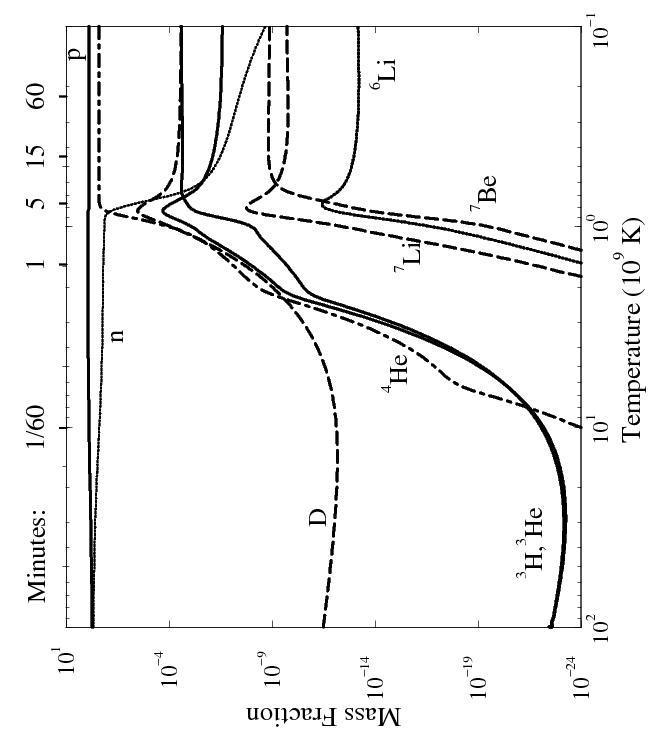
\includegraphics[width=\halfwidth,clip,trim={0 0 0 0},angle=270,origin=c]{Figures/Intro/BBNMassFraction.jpg}
		\caption{}
		\label{fig:BBNa}
	\end{subfigure}
	\begin{subfigure}[b]{\figurewidth}
		\centering
		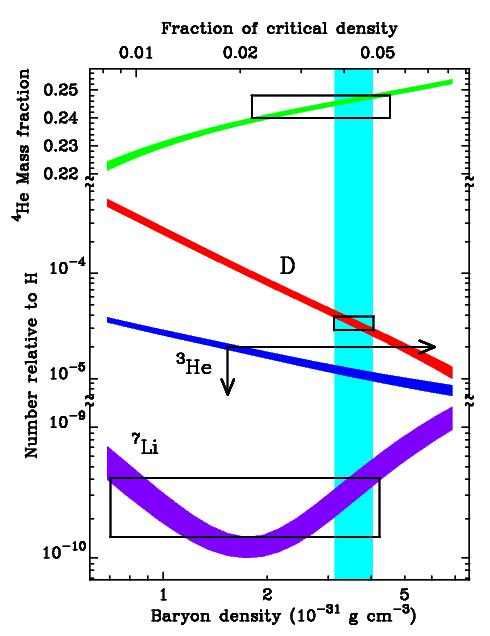
\includegraphics[width=\halfwidth,clip,trim={0 0 0 0}]{Figures/Intro/BBNBaryonDensity.jpg}
		\caption{}
		\label{fig:BBNb}
	\end{subfigure}
	\caption[Big Bang nucleosynthesis: mass fraction and abundance of nuclei]{(a) Mass fraction of nuclei as a function of temperature for $\eta_{10} = 5.1$. (b) Abundance of nuclei from BBN as a function of baryon density. Blue band shows the concordance region. Ref.~\cite{Tytler2000}} 
	\label{fig:BBN}
\end{figure}

The overall concordance on the figure provides a measure of the baryon density $\Omega_{B} =\num[separate-uncertainty=false]{0.040 +- 0.004} (95\% \text{CL})$ Ref.~\cite{Burles1998, Burles2001}. This value showed a great agreement with the measurement from the CMB. Both of them are together evidence for baryonic matter is not the only matter content in the universe.  

\subsection{The Cosmic Microwave Background}
The strongest cosmological evidence for existence of dark matter comes from the power spectrum of the measurements of the anisotropies of the cosmic Microwave Background(CMB). People can refer to Ref.~\cite{Olive2014} for better understanding of the CMB.

The CMB is electromagnetic radiation in the universe at the epoch of recombination, approximately $t_{dec} \num{\sim 3.8e5}$ years after the big bang Ref.~\cite{Jarosik2011}. It is an almost perfect isotropic Planck black body radiation at \SI{2.73}{\kelvin}. On top of the isotropic radiation, there are anisotropy features with amplitude \num{e-5} smaller than the amplitude of the isotropic components. The anisotropy features CMB provides evidence for the density fluctuation of the universe at the recombination epoch and evidence for dark matter.

The story of CMB start from the early stage of the universe. At that time the universe was opaque to photons due to the highly ionization medium in the universe. As the universe expand, the temperature of the universe eventually dropped below the ionization energy of an atom. Free electrons and nuclei combine into neutral atom. The universe became more transparent. Or in another word, photons started to decouple. This time is called recombination epoch. This transition region is also called the surface of photon last scattering. This "surface" is very "thin" in range of time, comparing to the duration of the life of universe before, and the relative temperature evolution is also small during that period. So the isotropic part of the photon spectrum look like a perfect Planck black body radiation. The expansion of the universe shift the wavelength of these photons with a redshift $z$, which is defined to be $z \equiv \frac{1}{a} - 1$. The temperature of the recombination is \SI{\sim 3000}{\kelvin}, corresponding redshift of $z=1100$. The relic temperature of the photon radiation is \SI{2.73}{\kelvin}, which is what we observe today.

Since the CMB reflects the photon emission at the small time range of recombination, it reveals the density fluctuation at that recombination time. This density fluctuation showed up in the anisotropic radiation spectrum. Fig.~\ref{fig:CMBSpectrum} shows the measure power spectrum of the anisotropic radiation. The power spectrum is the result of fitting the fluctuation ratio of temperature $\frac{\delta T}{T}$ with spherical harmonics. The amplitude for each $l$ indicates the Fourier transformation of the baryon density fluctuation. Smaller $l$ on the power spectrum correspond to large scale structures fluctuation, which lately may evolve to large scale structures in the universe, super clusters and voids. Larger $l$ on the power spectrum correspond to small scale structures, which lately may evolve into small scale structures in the universe, galaxies.  

\begin{figure}[htb]
	\centering
	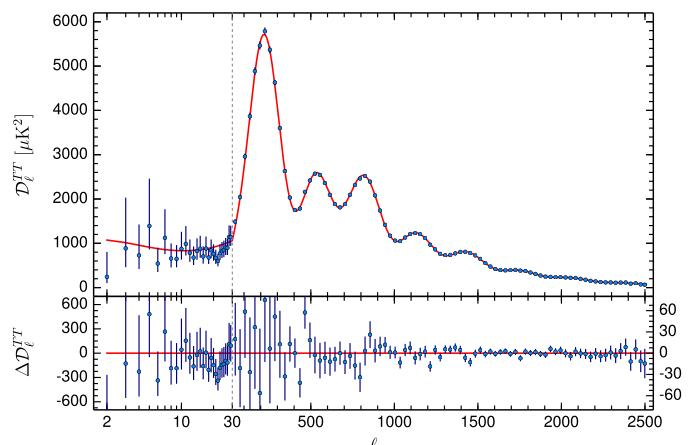
\includegraphics[width=\figurewidth,clip,trim={0 0 0 0},angle=0,origin=c]{Figures/Intro/CMBSpectrumTT.jpg}
	\caption[Temperature anisotropy spectrum of Cosmic Microwave Background]{Temperature anisotropy spectrum with the best fit to $\Lambda CDM$ model parameters from Planck 2016 measuremnt of the CMB. Ref.~\cite{Ade2016}}
	\label{fig:CMBSpectrum}
\end{figure}

The growing of density fluctuation under gravity can be derived from the combination Newtonian gravity and fluid dynamics. With joining Euler fluid equation, fluid continuity equation, and Poission equation of Newtonian gravity, one can derive the growing of density fluctuation $\delta_k$. 
\begin{align}
\label{density fluc grow}
\ddot{\delta_k} + 2 \frac{\dot{a}}{a} \dot{\delta_k} + (\frac{k^2 v_s^2}{a^2}-4 \pi G \rho) \delta_k = 0
\end{align}
here $\delta_k$ is the Flourier transformation of $\frac{\Delta \rho}{\rho}$, $\Delta \rho$ and $\rho$ are the density fluctuation and average density at certain moment. 

$v_s$ is the speed of sound wave. $v_s = \frac{\Delta P}{\Delta \rho} \sim \frac{1}{\sqrt{3}} $ for matter medium.

$k_J$ is the wave number satisfies
\begin{align}
\frac{k_J^2 v_s^2}{a^2}-4 \pi G \rho = 0  
\end{align}

For wave number $k \ll k_J$, Eqn.~\ref{density fluc grow} shows the solution of $\delta_k$ would not be stabilized by gravity. The corresponding comoving wavelength $\lambda_J = \frac{2 \pi}{k_J}$ of $k_J$ is called Jeans scale. Jeans mass $M_J$
\begin{align}
M_J = \frac{4 \pi \rho}{2} (\frac{\lambda_J}{2})^3
\end{align}
is the mass within Jeans scale. When the fluctuation scale exceeds Jeans scale or the mass contained in fluctuation exceeds Jeans mass, the system is not gravity stabilized.

Eqn.~\ref{density fluc grow} shows during the radiation dominant, the growing of matter fluctuation is slow. After the radiation matter equilibrium time $t_{eq}$, matter start dominant, the growth of matter fluctuation scale proportional to $a$. 

From the density fluctuation of today, $\delta \sim 1$, the derived density fluctuation at CMB time is \num{\sim e-3}. Comparing this value with the density fluctuation measured from the CMB, $\delta \num{\sim e-5}$, there is a clear discrepancy. This results in the proposing of dark matter. During the time between $t_{eq}$ (\SI{\sim e4}{\yr} from the Big Bang) and $t_{dec}$, baryons were still strongly coupled with photons. This results a larger $v_s$ for baryons. The growing of baryon density fluctuation is slower. At the same time, the growing dark matter density fluctuation is not influenced, still scales with $a$. The longer time for the density fluctuation to growth for dark matter results in a higher matter density fluctuation at the CMB time. This gives an explanation for the discrepancy. 

The recent measured baryon density, cold dark matter density, and the derived matter density from Planck satellite are $\Omega_B h^2= \num[separate-uncertainty=false]{0.02222 \pm 0.00023}$, $\Omega_C h^2 = \num[separate-uncertainty=false]{0.1199 \pm 0.0022}$, $\Omega_M = \num[separate-uncertainty=false]{0.316 \pm 0.014}$(with Hubble constant $h = \num[separate-uncertainty=false]{0.6726 \pm 0.0098}$), Ref.~\cite{Ade2016}: Table 1. This is a shocking result that showed the dominant component of matter in the universe is dark matter. The power spectrum shows a great fit with $\Lambda$CDM model, a universe with cold dark matter as the dark matter content. The discussion of cold dark matter and $\Lambda$CDM model will be in the next section. 

\subsection{Structure formation}
From the previous discussion, we know that the clustering of the matter in the universe is the result of instability of gravity. The small density fluctuation in the early time of the universe would grow to big density fluctuation over time. The structure formation of different scale is highly related to the initial density fluctuation spectrum and the time when the related physical scale $\lambda_f$ enter the event horizon $r_h(t)=\int_0^t \frac{1}{a(t')} dt'$. The great agreement between the simulations of the structure formation of the universe and the measurement of the structure formation of the real universe shows the advantage of cold dark matter and $\Lambda$CDM model.

Cold dark matter, warm dark matter Ref.~\cite{Peacock2003}, and hot dark matter are 

In the freeze-out model, the dark matter particle(here after as $X$) interacts with standard model particles, and the dark matter particle with its anti particle annihilate to standard model particles. Both dark matter particles and standard model particles are both created and achieved an equilibrium state as the early stage of universe. As the universe expands, the annihilation rate of the dark matter particle, which scale as $T^5$, dropped below the expansion rate, which scales as $T^2$. After then, the dark matter density will instead essentially drop with expansion of the universe and contribute to a relic density today. The time that annihilation rate reach expansion rate is called the decouple time of the dark matter. The correspond temperature is noted as $T_F$. 

Standard calculation for the relic density is estimated by the Boltzmann equation. The evolution of the number density of dark matter($n$) can be written as(Ref.~\cite{Bertone2005}, Eqn.~15),
\begin{align}
\frac{dn}{dt} + 3 H n = -\braket{\sigma v}(n^2-n_{eq}^2)
\end{align}
where $\sigma$ is the total annihilation cross section, $v$ is the velocity, and bracket denote the thermal average. $n_{eq}$ is the number density at thermal equilibrium. For massive particles, one has Maxwell-Boltzmann approximation of
\begin{align}
n_{eq}= g (\frac{mT}{2 \pi})^{3/2} e^{-m/T}
\end{align}
where $g$ is the degree of freedom.

$\braket{\sigma v}$ can be approximate in powers of $v^2$
\begin{align}
\braket{\sigma v} = a+b \braket{v^2} +\mathcal{O}(\braket{v^4}) \approx a+6b/x
\end{align}
where $x \equiv m/T$.

The solution of relic density today is (Ref.~\cite{Bertone2005}, Eqn.~26)
\begin{align}
\Omega_X h^2 \approx \frac{\SI{1.07e9}{\per\GeV}}{M_{pl}}\frac{x_F}{\sqrt{g_*}}\frac{1}{a+3b/x_F}
\end{align}
where $g*$ is the relativistic degree of freedom, $x_F$ is the value of $x$ at freeze out temperature.

For order of magnitude estimation, (Ref.~\cite{Bertone2005}, Eqn.~28)
\begin{align}
\Omega_X h^2 \approx \frac{\SI{3e-27}{\cm\cubed\per\second} }{\braket{\sigma v}}
\end{align}

Furthermore, if the mass of the dark matter particles are close to the mass of some standard model particles, the relic density can be changed by coannihilations, which is the resonance decay between the dark matter particles and standard model particles.

\section{Galactic Evidence of dark matter}
\subsection{Galactic Rotation Curves}
The galactic rotation curves are the almost earliest, and the most convincing observation results for the existence of dark matter. The measurement of the galactic rotation curves, which is the tangential velocity of stars about the galactic center as a function of their distance from the galactic center, show a plateau velocity after reach out a certain distance from the galactic center. As the acceleration due to gravity should go as $1/r^2$, the derived rotation velocity from the measurement of the luminous mass(stars, gas, nebulae, and other baryonic format matter) is much lower than the plateau velocity. This indicates that most galaxies are not composed primarily with luminous mass but with some other invisible mass. Oort Ref.~\cite{Oort1932} and Zwicky Ref.~\cite{Zwicky1933} separately gave the first measurement of this discrepancy. And this was the earliest hint of existence of dark matter relic in the galaxies. In the 1970s, the Rubin first firmly established the measurement of the rotation curves from the \SI{21}{\cm} line from stars of many galaxies Ref.~\cite{Rubin1983}, and confirm the need of dark matter for the explanation of the mass discrepancy. Fig.~\ref{fig:rotationCurves} shows the measured rotation curve from her work. 
 
\begin{figure}
	\centering
	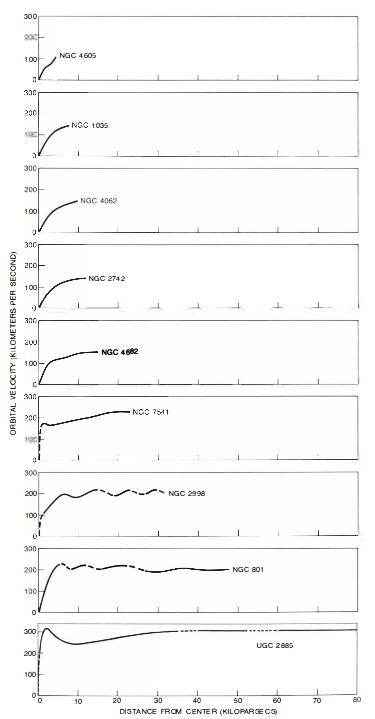
\includegraphics[width=0.7 \textwidth]{Figures/Intro/RotationCurveRubin.jpg}
	\caption[Rotation curve]{Rotation curve of 9 galaxies. Ref.~\cite{Rubin1983}.}
	\label{fig:rotationCurves}
\end{figure}

From the rotation curves Ref.~\cite{Rubin1983, Begeman1991}, the radii of the range of dark matter is much larger than the luminous mass. This indicates the difference of between the baryons mass and dark matter. Baryons are capable of losing energy with radiation, so it is easier for them to lose energy, slow down and then cluster together. However, for dark matter, which is assumed to be collisionless particles that interact primarily by gravity, similar physics process would be in much rate. So that the average velocity of dark matter is higher. The total mass of the dark matter in most galaxies are $~10$ times higher than the luminous matter. However, this ratio has a variance between different type of galaxies, and different clusters. Because of the difficulty of measuring the mass in the center of the galaxies, it gains uncertainty for the distribution of the mass profile of dark matter in the galaxies. The most common model proposed for the mass profile by Navarro, Frenk, \& White (1996, 1997, here after NFW),
\begin{align}
\rho_{DM}= \frac{\delta_c \rho_{crit}}{(r/r_s)(1+r/r_s)^2}
\end{align}
where $\rho_{crit}$ is the critical density of the universe, and $\delta_c$ and $r_s$ are the concentration parameter and the scaled radius Ref.~\cite{Navarro1996, Navarro1997}. 

An alternative explanation for the rotation curve is modified Newtonian dynamics(MOND) at low acceleration scale Ref.~\cite{Milgrom1983, Milgrom1983a, Milgrom1983b}. The theory is motivated by explaining the challenges in $\Lambda CDM$ model Ref.~\cite{Famaey2012}.However, evidence supporting or rejecting this physics in lab has not been reported. 

%\section{Other Observations}
%\SI{3.55}{\keV} annillation line observe for multiple galaxy X-ray spectrum
%\paragraph{Weak lensing}
%\paragraph{X-ray spectrum abnormally}
%----------------------------------------------------------------------------------------
%%	SECTION 2
%%----------------------------------------------------------------------------------------
%\section{Evidence of Dark Matter}
%\subsection{}
%\subsection{Gravitational lensing}
%\subsection{Dark matter in clusters, galaxies}
%%----------------------------------------------------------------------------------------
%%	SECTION 3
%%----------------------------------------------------------------------------------------
%\section{Dark matter candidates}
%\subsection{Neutrinos}
%\subsection{macho,super massive blackholes}
%\subsection{WIMP}
